% This is samplepaper.tex, a sample chapter demonstrating the
% LLNCS macro package for Springer Computer Science proceedings;
% Version 2.21 of 2022/01/12
%
\documentclass[runningheads]{llncs}
%
\usepackage[T1]{fontenc}
% T1 fonts will be used to generate the final print and online PDFs,
% so please use T1 fonts in your manuscript whenever possible.
% Other font encondings may result in incorrect characters.
%
\usepackage{graphicx}
% Used for displaying a sample figure. If possible, figure files should
% be included in EPS format.
%
% If you use the hyperref package, please uncomment the following two lines
% to display URLs in blue roman font according to Springer's eBook style:
%\usepackage{color}
%\renewcommand\UrlFont{\color{blue}\rmfamily}

\usepackage{geometry}
\usepackage{xcolor}
\usepackage{booktabs,tabularx}
\usepackage{hyperref}

\usepackage{xspace}
\newcommand{\thesystem}{\textit{HarmoniKt}\xspace}

\usepackage{acronym}
\acrodef{iiot}[IIoT]{Industrial Internet of Things}
\acrodef{mir}[MiR]{Mobile Industrial Robots}
\acrodef{spot}[SPOT]{Boston Dynamics Spot}

%
\begin{document}
%
\title{HarmoniKt: Microservices Middleware for\\Heterogeneous Robot Fleet Management\\
\small\textnormal{
    Project Report for the PhD Course \emph{Service Orchestration and Industrial IoT Platforms for Industry 4 and 5.0 environments} (A.Y. 2024/2025)
}
}
%
%\titlerunning{Abbreviated paper title}
% If the paper title is too long for the running head, you can set
% an abbreviated paper title here
%
\author{
Manuel Andruccioli\inst{1} \and
Angela Cortecchia\inst{1} \and
\\
Davide Domini\inst{1} \and
Nicolas Farabegoli\inst{1}
}
%
\authorrunning{M. Andruccioli et al.}
% First names are abbreviated in the running head.
% If there are more than two authors, 'et al.' is used.
%
\institute{
University of Bologna, Department of Computer Science and Engineering, Italy
\\
\email{\{manuel.andruccioli,angela.cortecchia,davide.domini,nicolas.farabegoli\}@unibo.it}
}
%
\maketitle              % typeset the header of the contribution
%
\begin{abstract}
This report presents a comprehensive analysis of \thesystem, a microservices-based middleware solution designed to provide unified access to heterogeneous robot fleets in \ac{iiot} contexts. The project successfully integrates \ac{spot} and \ac{mir} through a modular architecture that abstracts robot-specific functionalities behind standardized APIs. This analysis examines the project's architecture, implementation details, development evolution, and technical achievements.

\keywords{Microservices \and Middleware \and Robot Management.}
\end{abstract}
%
%
%
\section{Project Goal}

\thesystem aims to provide a comprehensive solution for robot fleet management middleware, addressing the complex challenge of heterogeneous robot integration in modern industrial environments. The project serves as a demonstration of advanced software engineering practices through its sophisticated microservices architecture, comprehensive API design, and innovative multi-language implementation approach.

The project's success can be measured through several key achievements:

\begin{itemize}
    \item \textbf{Unified API Design}: successfully abstracts diverse robot functionalities through standardized REST APIs
    \item \textbf{Multi-Technology Integration}: seamlessly combines Kotlin-based services with Python-based robot interfaces
    \item \textbf{Scalable Architecture}: implements microservices pattern enabling easy addition of new robot types
    \item \textbf{Production-Ready Infrastructure}: includes containerization, service discovery, and reverse proxy configuration
\end{itemize}

%
%
%
\section{Project Objectives}

\thesystem represents a comprehensive approach to modular and scalable middleware for integrating robots of different brands and models. The system provides users with a consistent and standardized interface for interacting with machines regardless of their manufacturer, effectively solving one of the most pressing challenges in modern industrial automation.

The core objectives demonstrate our commitment to creating a robust and flexible system:

\begin{enumerate}
    \item \textbf{Abstraction Layer}: create a unified interface that abstracts robot-specific implementation details
    \item \textbf{Interoperability}: enable seamless integration between different robot types and brands
    \item \textbf{Scalability}: design architecture that supports easy integration of new robot models
    \item \textbf{Standardization}: establish common APIs for robot status monitoring and control
\end{enumerate}

%
%
%
\section{Architecture Analysis}

\subsection{Microservices Design Pattern}

The project embraces a distributed microservices architecture philosophy with clear separation of concerns, ensuring that each component has a well-defined responsibility and can operate independently. This architectural approach provides several advantages including improved maintainability, better fault isolation, and enhanced scalability.

\begin{table}[htbp]
\centering
\begin{tabular}{@{}lp{10cm}@{}}
\toprule
\textbf{Service} & \textbf{Responsibility} \\
\midrule
\textbf{robot-service} & Central orchestration service providing unified APIs \\
\textbf{spot-service} & Boston Dynamics Spot robot integration (Python-based) \\
\textbf{mir-service} & MiR robot integration (Kotlin-based) \\
\textbf{map-service} & Spatial data and mapping functionality management \\
\textbf{group-mission-service} & Multi-robot coordination and mission planning \\
\textbf{service-registry} & Service discovery and health monitoring \\
\bottomrule
\end{tabular}
\caption{Microservices Architecture Components}
\label{tab:services}
\end{table}

The \textbf{robot-service} acts as the central orchestration hub, providing unified APIs that abstract the complexity of individual robot implementations. This service ensures that clients interact with a consistent interface regardless of the underlying robot types. The \textbf{spot-service} demonstrates our commitment to leveraging the best tools for each specific task, utilizing Python to take full advantage of Boston Dynamics' official SDK. In contrast, the \textbf{mir-service} showcases our Kotlin-based approach, highlighting the flexibility of our polyglot architecture.

\begin{figure}[htbp]
    \centering
    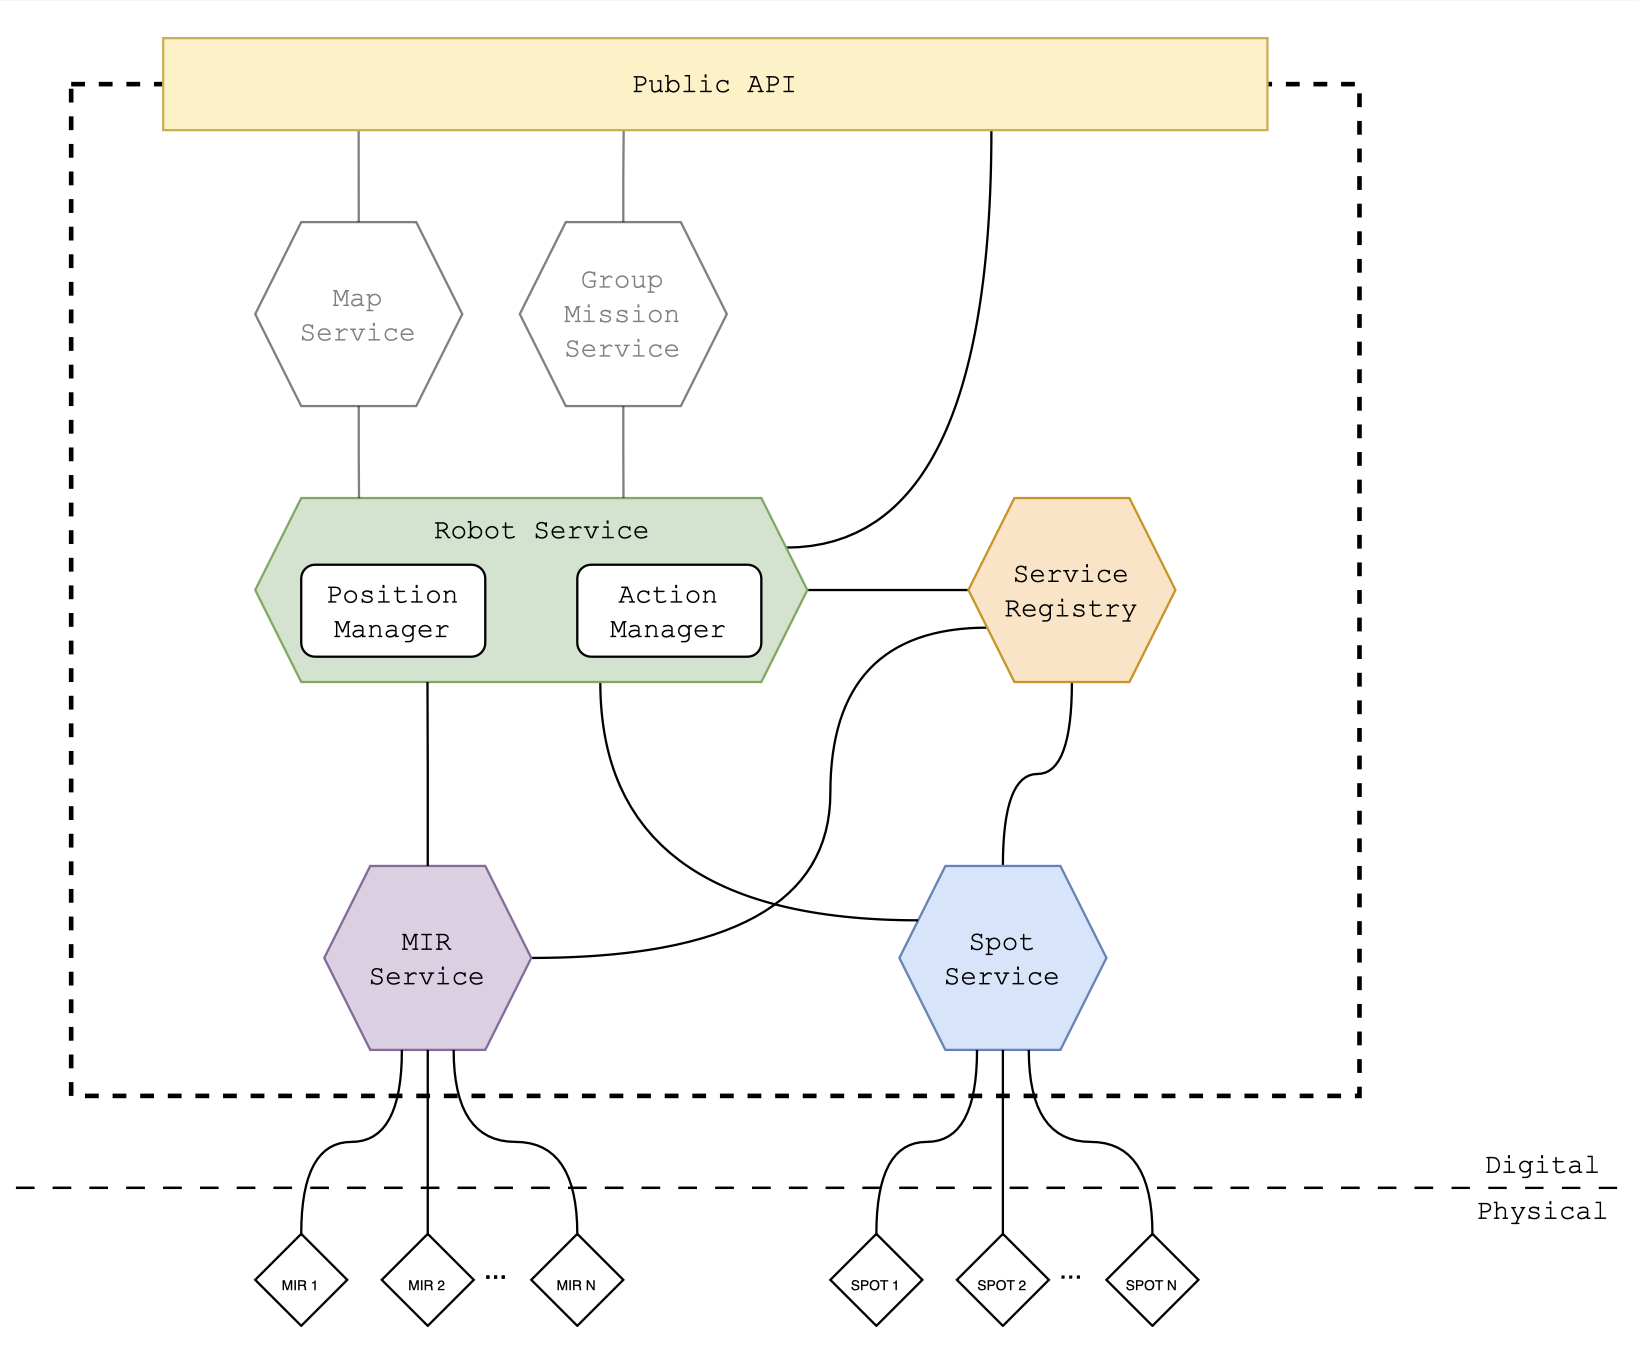
\includegraphics[width=0.7\textwidth]{img/harmonikt-architecture.png}
    \caption{High-Level Architecture Diagram}
    \label{fig:architecture}
\end{figure}

The \textbf{map-service} handles all spatial data and mapping functionality, providing essential navigation and localization services that multiple robots can share. The \textbf{group-mission-service} enables sophisticated multi-robot coordination and mission planning, allowing for complex orchestrated operations across different robot types. Finally, the \textbf{service-registry} implements comprehensive service discovery and health monitoring, ensuring that the distributed system remains resilient and self-healing.

\subsection{Technology Stack}

The project demonstrates a thoughtful polyglot programming approach, selecting the most appropriate technology for each specific requirement. Our technology choices reflect a balance between modern development practices and practical integration needs:

\begin{itemize}
    \item \textbf{Primary Language}: Kotlin with Ktor framework\footnote{\url{https://ktor.io}}
    \item \textbf{Robot-Specific Integration}: Python for Boston Dynamics SDK
    \item \textbf{API Documentation}: OpenAPI 3.1.1 Specification\footnote{\url{https://spec.openapis.org/oas/v3.1.1.html}}
    \item \textbf{Containerization}: Docker Compose for service orchestration\footnote{\url{https://docs.docker.com/compose/}}
    \item \textbf{Service Discovery}: Consul\footnote{\url{https://consul.io/}}
    \item \textbf{Reverse Proxy}: Caddy server\footnote{\url{https://caddyserver.com}}
\end{itemize}

Kotlin with the Ktor framework serves as our primary development language, chosen for its excellent type safety, concise syntax, and robust ecosystem. The decision to use Kotlin reflects our commitment to modern, maintainable code while leveraging the mature JVM ecosystem. For robot-specific integration, we strategically employ Python when interfacing with the Boston Dynamics SDK, recognizing that using the manufacturer's preferred language and official libraries provides the most reliable and feature-complete integration possible.

%
%
%
\subsection{Infrastructure Components}

The infrastructure foundation relies on several key components that ensure maintainability and operational excellence:

\begin{itemize}
    \item \textbf{Build System}: Gradle with Kotlin DSL
    \item \textbf{Dependency Management}: Renovate bot for automated updates
    \item \textbf{CI/CD}: GitHub Actions integration
    \item \textbf{Release Management}: Semantic versioning with automated releases
\end{itemize}

The build system utilizes Gradle with Kotlin DSL, providing a modern, type-safe approach to build configuration that integrates seamlessly with our Kotlin codebase. Dependency management is automated through Renovate bot, which continuously monitors for updates and creates pull requests for dependency upgrades, ensuring that our codebase remains secure and up-to-date without manual intervention.

%
%
%
\section{API Design and Specification}

\subsection{REST API Structure}

The unified API adheres strictly to RESTful principles with clear resource hierarchies that make the interface intuitive and predictable for developers. The API design emphasizes consistency, ensuring that similar operations across different resource types follow identical patterns and conventions.

\subsubsection{Robot Management Endpoints}

The robot management functionality provides comprehensive lifecycle management for robotic assets within the system:

\begin{itemize}
    \item \texttt{GET /robots} - Retrieve all active robots
    \item \texttt{POST /robots} - Register new robot
    \item \texttt{GET /robots/\{robotId\}} - Get robot status
    \item \texttt{DELETE /robots/\{robotId\}} - Unregister robot
    \item \texttt{POST /robots/\{robotId\}/actions} - Execute robot action
\end{itemize}

\subsubsection{Point of Interest (POI) Management}

The POI management system provides spatial context and navigation targets for robot operations:

\begin{itemize}
    \item \texttt{GET /pois} - List all points of interest
    \item \texttt{POST /pois} - Create new POI
    \item \texttt{GET /pois/\{poiId\}} - Get POI details
    \item \texttt{DELETE /pois/\{poiId\}} - Remove POI
\end{itemize}

\subsubsection{Marker Management}

The marker management functionality provides fine-grained control over POI-associated navigation and reference points:

\begin{itemize}
    \item \texttt{GET /pois/\{poiId\}/markers} - List POI markers
    \item \texttt{POST /pois/\{poiId\}/markers} - Add marker to POI
    \item \texttt{GET /pois/\{poiId\}/markers/\{markerId\}} - Get specific marker
    \item \texttt{DELETE /pois/\{poiId\}/markers/\{markerId\}} - Remove marker
\end{itemize}

%
%
%
\section{Implementation Analysis}

\subsection{Code Organization}

The project follows clean architecture principles with clear separation of concerns, ensuring that code remains maintainable and testable as the system grows in complexity. This architectural approach facilitates understanding and modification by organizing code into logical layers with well-defined responsibilities.

\subsubsection{Common Module}

The common module serves as the foundation for the entire system, containing shared components that are utilized across multiple services:

\begin{itemize}
    \item \textbf{Model Layer}: Core domain objects (Robot, Action, Marker, POI)
    \item \textbf{Repository Layer}: Data access abstractions
    \item \textbf{DTO Layer}: API data transfer objects
    \item \textbf{Utilities}: Consul integration and Ktor setup
\end{itemize}

\subsubsection{Service-Specific Implementation}

Each microservice follows consistent architectural patterns that promote code reusability and reduce cognitive load for developers working across different services:

\begin{itemize}
    \item \textbf{API Layer}: HTTP endpoint definitions
    \item \textbf{Handler Layer}: Request processing logic
    \item \textbf{Repository Layer}: Data persistence and external service integration
    \item \textbf{Resource Layer}: Static data and configuration
\end{itemize}

%
%
%
\subsection{Quality Assurance}

The project demonstrates a strong commitment to code quality through multiple automated and manual quality assurance mechanisms:

\begin{itemize}
    \item \textbf{Linting}: ktlint integration for Kotlin code style
    \item \textbf{Pre-commit Hooks}: Automated code quality checks
    \item \textbf{Documentation}: Comprehensive KDoc documentation
    \item \textbf{Testing}: Mock repository implementations for testing
\end{itemize}

Kotlin code style consistency is maintained through ktlint integration, which automatically enforces coding standards and prevents style inconsistencies from being introduced into the codebase. Pre-commit hooks provide automated code quality checks that run before code is committed to version control, catching potential issues early in the development process.

%
%
%
\section{Technical Innovations}

%
%
%
\subsection{Multi-Language Integration}

One of the most significant technical achievements of the project is the successful integration of different programming languages within a cohesive system architecture. This polyglot approach allows us to leverage the specific strengths of each language and ecosystem while maintaining system coherence.

The Kotlin services take full advantage of the JVM ecosystem and provide excellent type safety, enabling us to catch many potential errors at compile time rather than runtime. Meanwhile, our Python integration strategy allows us to utilize the Boston Dynamics official SDK in its native environment, ensuring that we have access to all features and receive optimal support from the manufacturer. The seamless communication between these different language environments is achieved through HTTP-based service interaction, which provides a language-agnostic integration mechanism that is both reliable and well-understood.

%
%
%
\subsection{Service Discovery}

The Consul integration provides sophisticated service discovery capabilities that are essential for operating a distributed microservices architecture. Dynamic service registration ensures that services can find and communicate with each other automatically, without requiring manual configuration or hardcoded service locations. Health monitoring functionality continuously tracks the status of all services, enabling the system to automatically route traffic away from unhealthy services and provide early warning of potential issues. The load balancing capabilities distribute requests intelligently across multiple service instances, ensuring optimal resource utilization and improved system resilience.

%
%
%
\section{Deployment and Operations}

%
%
%
\subsection{Containerization Strategy}

The containerization approach emphasizes both efficiency and maintainability, ensuring that services can be deployed consistently across different environments:

\begin{itemize}
    \item \textbf{Optimized Images}: Multi-stage builds for minimal image size
    \item \textbf{Configuration Management}: Environment-based configuration
    \item \textbf{Orchestration}: Docker Compose for development environments
\end{itemize}

Each service is containerized using carefully crafted Docker images that utilize multi-stage builds to minimize final image size while maintaining all necessary functionality. This approach reduces deployment times, storage requirements, and attack surface area.

%
%
%
\subsection{Reverse Proxy Configuration}

The Caddy server implementation provides sophisticated reverse proxy functionality that serves as the primary entry point for all external requests:

\begin{itemize}
    \item \textbf{Request Routing}: Intelligent request distribution
    \item \textbf{SSL Termination}: Automatic HTTPS certificate management
    \item \textbf{API Gateway Functionality}: Centralized access point
\end{itemize}

The request routing capabilities intelligently distribute incoming requests to the appropriate backend services based on URL patterns and other criteria, ensuring that clients can access all system functionality through a single, consistent interface.

\section{Challenges and Solutions}

\subsection{Heterogeneous Integration Challenges}

One of the most significant challenges encountered during development was dealing with the fundamental differences in robot APIs and communication protocols. Different manufacturers implement vastly different approaches to robot control, status reporting, and configuration management, making it difficult to create a unified interface that doesn't sacrifice functionality or introduce artificial limitations.

Our solution centered around developing a sophisticated abstraction layer that uses standardized Data Transfer Objects (DTOs) to create a common language for robot interaction. This approach allows us to preserve the unique capabilities of each robot type while presenting a consistent interface to client applications.

\subsection{Technology Diversity}

Managing a multi-language codebase presents unique challenges in terms of tooling, build processes, testing strategies, and developer onboarding. Each language brings its own ecosystem, dependencies, and best practices, which can create complexity when trying to maintain consistency across the entire project.

The microservices architecture provides an elegant solution to this challenge by establishing clear service boundaries that allow different languages to coexist without interference. Each service can utilize the most appropriate technology stack while communicating with other services through well-defined HTTP APIs.

\subsection{API Consistency}

Maintaining consistent API behavior across different robot types proved challenging because each robot manufacturer provides different capabilities, status information, and control mechanisms. Creating a unified API that doesn't become either overly generic or overly specific required careful design consideration.

Our solution involved developing comprehensive OpenAPI specifications that define the expected behavior for all API endpoints, combined with polymorphic design patterns that allow for robot-specific extensions while maintaining core consistency.

\section{Future Extensibility}

\subsection{New Robot Integration}

The architecture has been specifically designed to facilitate the addition of new robot types with minimal disruption to existing functionality. The integration process follows a well-defined pattern:

\begin{enumerate}
    \item Implement robot-specific service following established patterns
    \item Extend DTO definitions for robot-specific features
    \item Add authentication mechanisms as needed
    \item Register with service discovery
\end{enumerate}

\subsection{Feature Enhancement Opportunities}

Several areas present exciting opportunities for future development and enhancement:

\begin{itemize}
    \item \textbf{Advanced Mission Planning}: Multi-robot coordination algorithms
    \item \textbf{Real-time Monitoring}: WebSocket-based status streaming
    \item \textbf{Analytics Integration}: Robot performance metrics and analytics
    \item \textbf{Security Enhancements}: OAuth2/JWT authentication
\end{itemize}

Advanced mission planning capabilities could implement sophisticated multi-robot coordination algorithms that enable complex collaborative tasks and optimize resource utilization across the entire fleet. Real-time monitoring functionality using WebSocket-based status streaming would provide instant updates on robot status and mission progress, enabling more responsive control systems and better situational awareness.

\section{Development Evolution}

The project evolved through several distinct phases, each building upon the foundations established in previous iterations. The following sections outline the key activities and contributions of each group member during these developmental phases, demonstrating how the collaborative effort resulted in the comprehensive system described in this report.

%
%
%
\subsubsection{Foundation Phase (March - May 2025)}

\begin{itemize}
    \item Visits to BI-REX Competence Center\footnote{\url{https://bi-rex.it/en/}} for requirements gathering and robot capabilities analysis (Manuel, Angela, Davide, Nicolas)
    \item Initial project setup and architecture definition (Manuel, Angela, Davide, Nicolas)
    \item Basic robot interface and action model establishment (Manuel, Angela, Davide, Nicolas)
    \item Build system configuration and CI/CD pipeline setup (Manuel, Angela, Davide, Nicolas)
\end{itemize}

%
%
%
\subsubsection{Core Development Phase (June 2025)}

\begin{itemize}
    \item Implementation of marker and point-of-interest management (Manuel, Angela)
    \item Robot registration and status monitoring functionality (Davide, Nicolas)
    \item Consul service discovery integration (Nicolas)
    \item Docker containerization setup (Manuel, Nicolas)
\end{itemize}

%
%
%
\subsubsection{Integration Phase (July 2025)}

\begin{itemize}
    \item Spot robot service implementation in Python (Manuel, Davide)
    \item MiR robot service development (Angela, Davide)
    \item API standardization and OpenAPI specification (Manuel, Angela, Nicolas)
    \item Swagger UI integration for API documentation (Manuel, Angela, Davide)
\end{itemize}

%
%
%
\subsubsection{Refinement Phase (August 2025)}

\begin{itemize}
    \item POI and marker API enhancements (Angela)
    \item Caddy reverse proxy integration (Manuel)
    \item Code quality improvements and documentation (Nicolas)
    \item Bug fixes and API consistency improvements (Davide)
\end{itemize}



%
% ---- Bibliography ----
%
% BibTeX users should specify bibliography style 'splncs04'.
% References will then be sorted and formatted in the correct style.
%
% \bibliographystyle{splncs04}
% \bibliography{mybibliography}
%
% \begin{thebibliography}{8}
% \bibitem{ref_article1}
% Author, F.: Article title. Journal \textbf{2}(5), 99--110 (2016)

% \bibitem{ref_lncs1}
% Author, F., Author, S.: Title of a proceedings paper. In: Editor,
% F., Editor, S. (eds.) CONFERENCE 2016, LNCS, vol. 9999, pp. 1--13.
% Springer, Heidelberg (2016). \doi{10.10007/1234567890}

% \bibitem{ref_book1}
% Author, F., Author, S., Author, T.: Book title. 2nd edn. Publisher,
% Location (1999)

% \bibitem{ref_proc1}
% Author, A.-B.: Contribution title. In: 9th International Proceedings
% on Proceedings, pp. 1--2. Publisher, Location (2010)

% \bibitem{ref_url1}
% LNCS Homepage, \url{http://www.springer.com/lncs}. Last accessed 4
% Oct 2017
% \end{thebibliography}
\end{document}
